%%%%%%%%%%%%%%%%%%%%%%%%%%%%% Define Article %%%%%%%%%%%%%%%%%%%%%%%%%%%%%%%%%%
\documentclass[12pt]{article}

%%%%%%%%%%%%%%%%%%%%%%%%%%%%% Using Packages %%%%%%%%%%%%%%%%%%%%%%%%%%%%%%%%%%
\usepackage{geometry}
\usepackage{amsmath}
\usepackage[utf8]{inputenc}
\usepackage{graphicx}
\usepackage{pythontex}
\usepackage{booktabs}
\usepackage{caption}

%%%%%%%%%%%%%%%%%%%%%%%%%%%%% other settings %%%%%%%%%%%%%%%%%%%%%%%%%%%%%%%%%%
\DeclareMathOperator{\E}{\mathbb{E}}
\setlength{\parindent}{1em}
\setlength{\parskip}{1em}
\renewcommand{\baselinestretch}{1.15}

%%%%%%%%%%%%%%%%%%%%%%%%%%%%%%%% Page Setting %%%%%%%%%%%%%%%%%%%%%%%%%%%%%%%%%
\geometry{
    a4paper,
    total={170mm,257mm},
    left=20mm,
    top=20mm,
}

%%%%%%%%%%%%%%%%%%%%%%%%%%%%%%%% Py settings  %%%%%%%%%%%%%%%%%%%%%%%%%%%%%%%%%%
\begin{pycode}
    import pandas as pd
    from pathlib import PurePath
    import os
    import sys
    main_dir = os.path.dirname(os.getcwd())
    sys.path.append(main_dir)
    os.chdir(main_dir)

    from TSEMonthlySale import ns


    cte = ns.Constants()
    td = ns.TexDataFilenames()
    dirs = ns.Dirs()


    texDtDir = dirs.texdata
    varfn = td.vars
    varpn = texDtDir / f"{varfn}.csv"
    fi = PurePath(varpn)

    # vars = pd.read_csv(varpn, index_col = 0, )

    bslbl = cte.Balanced
    wslbl = cte.Whole

\end{pycode}

%%%%%%%%%%%%%%%%%%%%%%%%%%%%%%% Title & Author %%%%%%%%%%%%%%%%%%%%%%%%%%%%%%%%
\title{TSE Monthly Sale Project \\ A Brief Report}
\author{Mahdi Mir}
\date{}


%%%%%%%%%%%%%%%%%%%%%%%%%%%%%%% Document beginning %%%%%%%%%%%%%%%%%%%%%%%%%%%%
\begin{document}
    \maketitle
    \date
%%%%%%%%%%%%%%%%%%%%%%%%%%%%%%%%%%%%%%%%%%%%%%%%%%%%%%%%%%%%%%%%%%%%%%%%%%%%%%%


    \section{Files and Folders}

    In the folder delivered, there is the current report and three folders named: `code', `data', and `figs'.

    \subsection{Code}
    In the code folder, we have all the codes for the project. These codes essentially extract monthly data from `codal.ir' each time they are executed.
    The code extracts all monthly sales data from the beginning of monthly sale reports to the latest available monthly sale statement.

    \subsection{data}
    The complete extracted monthly sale data and its balanced subsample are in the data folder. Moreover there are bunch of other output datasets which are deducted from the sale data and some analysis about it.

    \subsection{figs}
    In this folder, all the following charts and more are available as quality '.eps' files.


    \section{Data Description}

    \begin{pycode}
        sumstat_fn = td.sumStat
        ss = ns.SumStatCols()
        stat = pd.read_csv(fi.with_stem(sumstat_fn), index_col=0)
    \end{pycode}
    \newcommand{\st}[2]{\py{stat.loc[#1, #2]}}

    In the following table, I present a set of descriptive numbers about the data and its balanced subsample. The balanced subsample starts from \st{bslbl}{ss.initJMonth} until the latest month.
    The whole sample consists of only two types of firms: production and service.

    \begin{table}
        \small \setlength{\tabcolsep}{4pt}
        \captionsetup{font=large}
        \caption{Datasets Description}

        \begin{center}
            \begin{tabular}{lcc}
                \toprule
                & Whole Sample                                       & The Balanced Subsample-\st{bslbl}{ss.initJMonth}   \\
                \midrule
                Observations              & \st{wslbl}{ss.obs}                                 & \st{bslbl}{ss.obs}                                 \\
                Initial Month             & \st{wslbl}{ss.initJMonth}                          & \st{bslbl}{ss.initJMonth}                          \\
                Last Month                & \st{wslbl}{ss.lastJMonth}                          & \st{bslbl}{ss.lastJMonth}                          \\
                Months Count              & \st{wslbl}{ss.monthsNo}                            & \st{bslbl}{ss.monthsNo}                            \\
                Mean Observations Monthly & \py{round(stat.loc[wslbl,ss.avgObsMonthly],1)}     & \py{round(stat.loc[bslbl,ss.avgObsMonthly])}       \\
                Firms Number              & \st{wslbl}{ss.firmsNo}                             & \st{bslbl}{ss.firmsNo}                             \\
                Production Firms          & \st{wslbl}{ss.productionNo}                        & \st{bslbl}{ss.productionNo}                        \\
                Prdocution Firms \%       & \py{round(stat.loc[wslbl,ss.productionPct]*100,1)} & \py{round(stat.loc[bslbl,ss.productionPct]*100,1)} \\
                \bottomrule
            \end{tabular}
        \end{center}
    \end{table}

    The data for the above table can be accessed through the `data' folder.

    \subsection{Firms Lists}
    The `data' folder contains two lists of firms for each of complete sample and the balanced subsample.


    \section{Monthly Aggregate}
    For each of the whole sample and the balanced subsample monthly aggregates and statistics are calculated. These two monthly data are saved in the `data' folder as two distinct `Excel' files.

    \subsection{Figures}
    This section proposes some charts regarding monthly aggregates abour the whole and the balanced subsample.

    \subsubsection{Unique Firms Count}

    \begin{figure}
        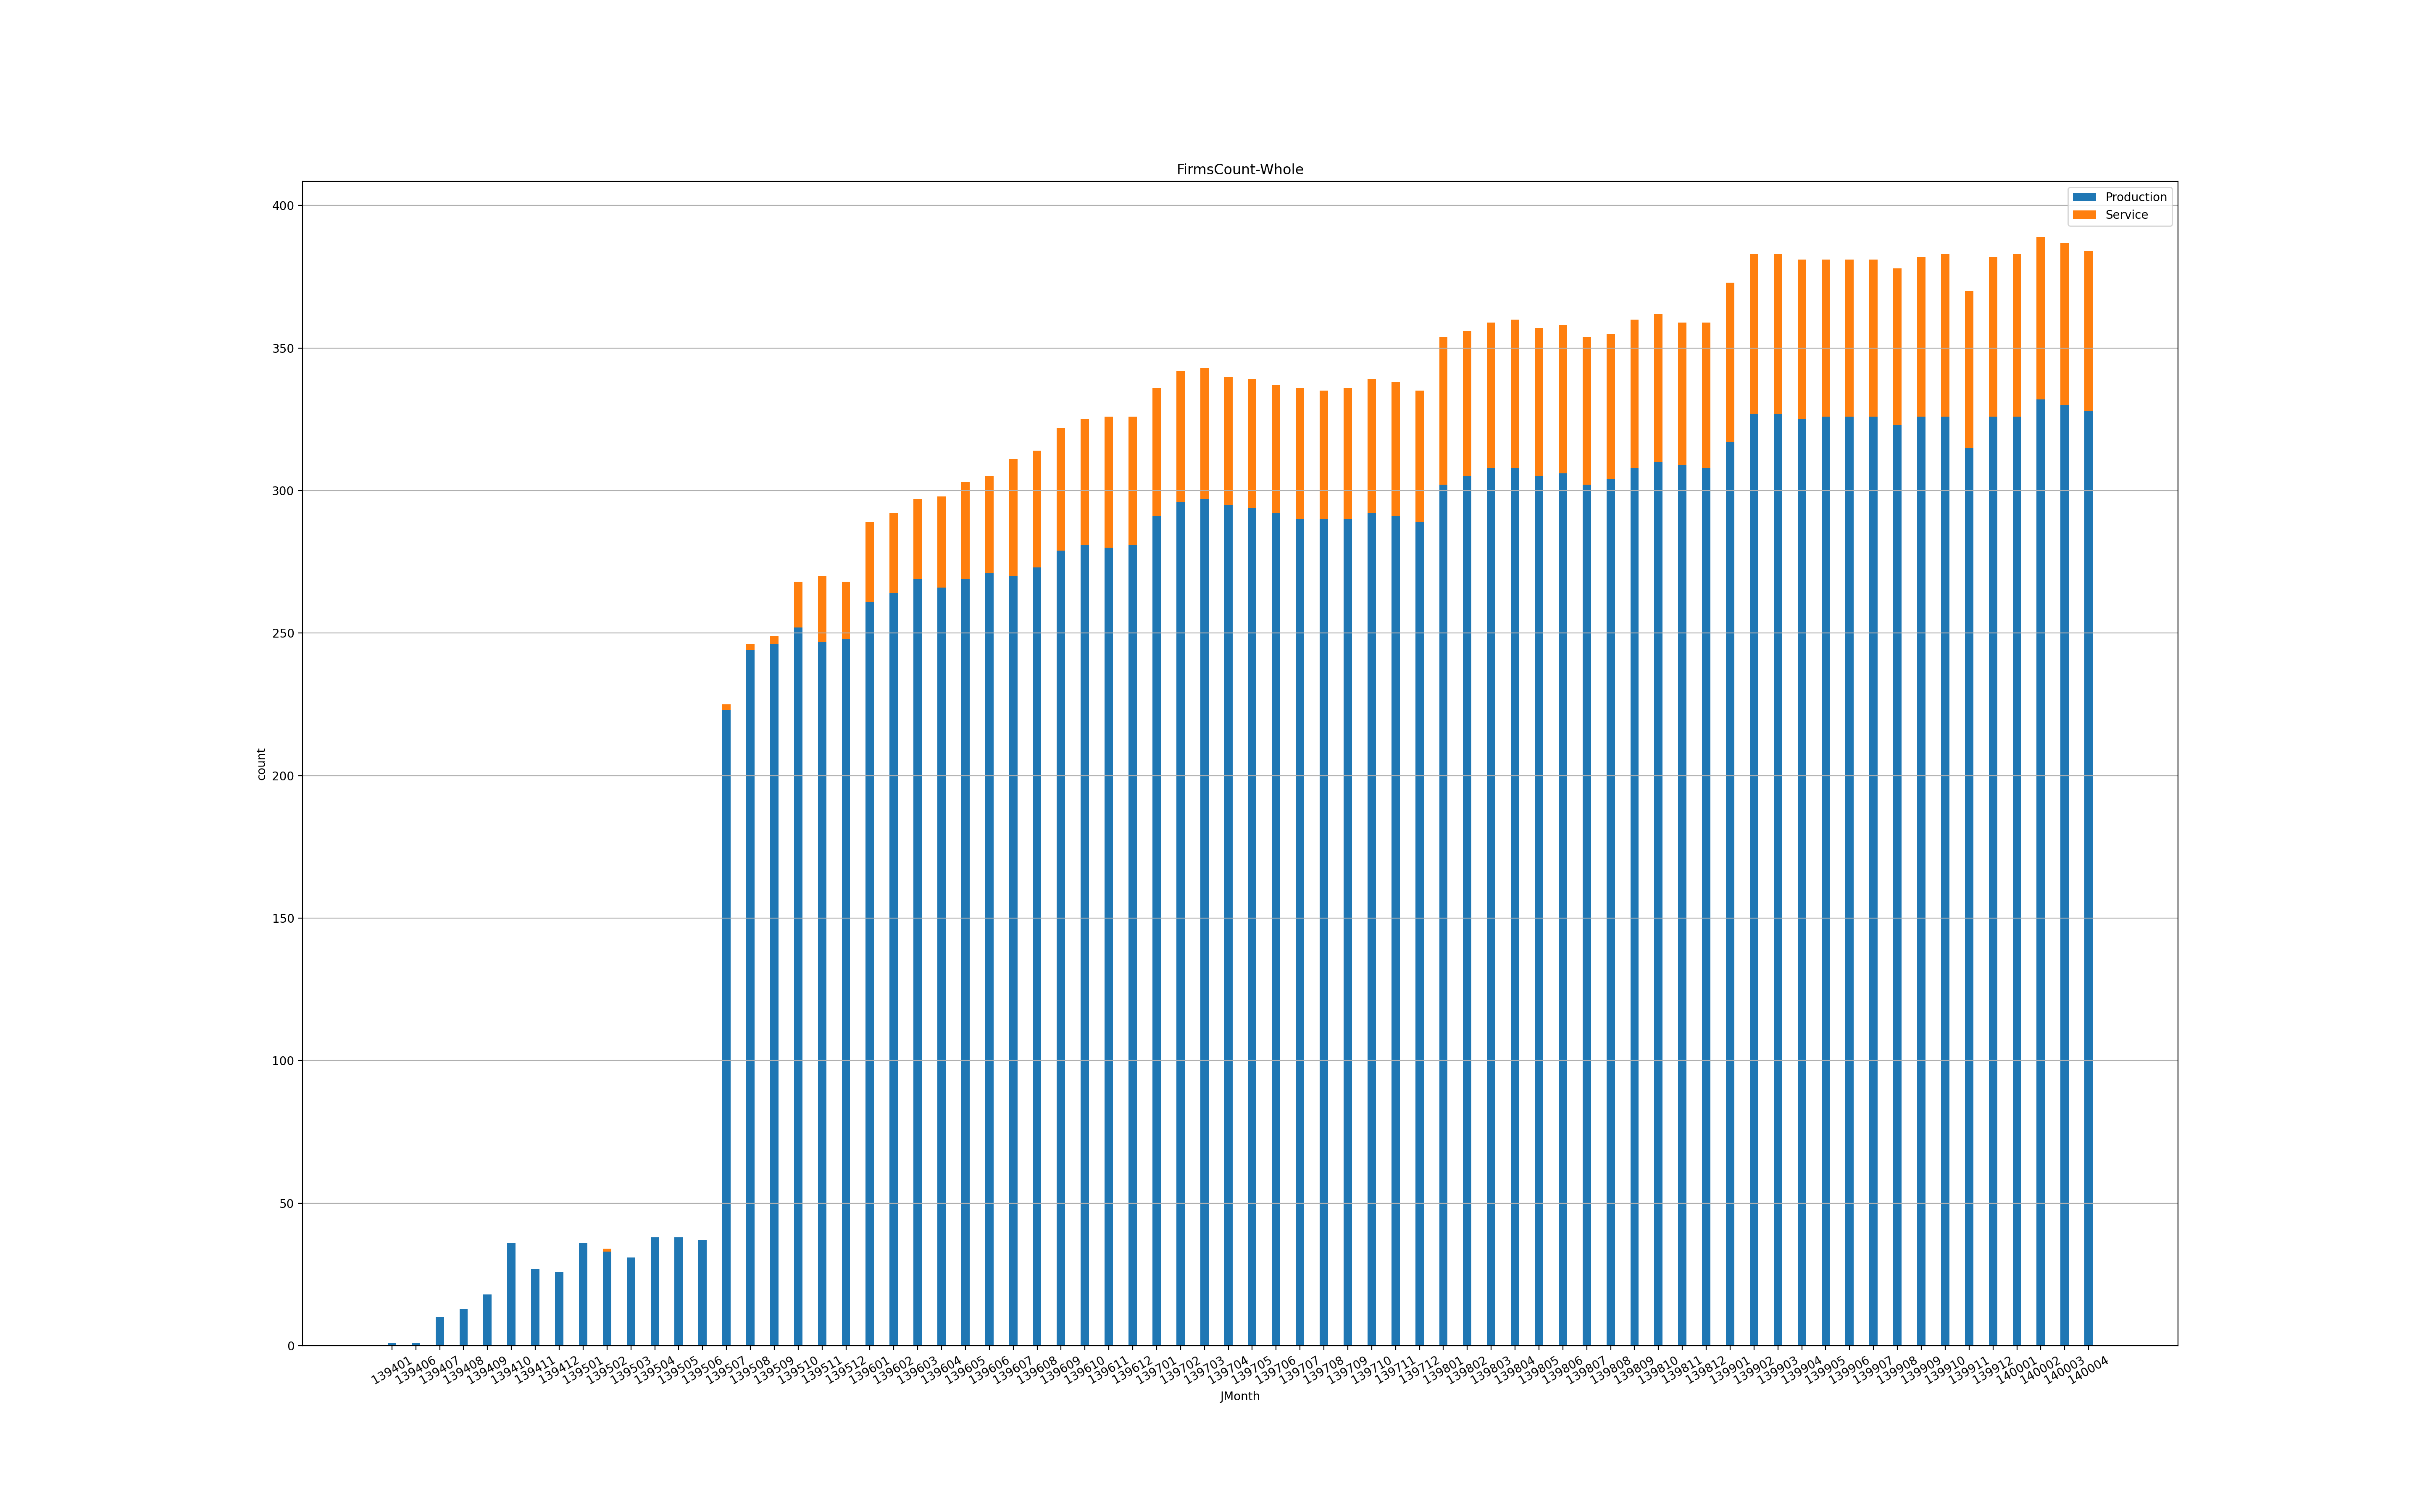
\includegraphics[width=\linewidth]{../data/figs/FirmsCount-Whole.png}
    \end{figure}
    \begin{figure}
        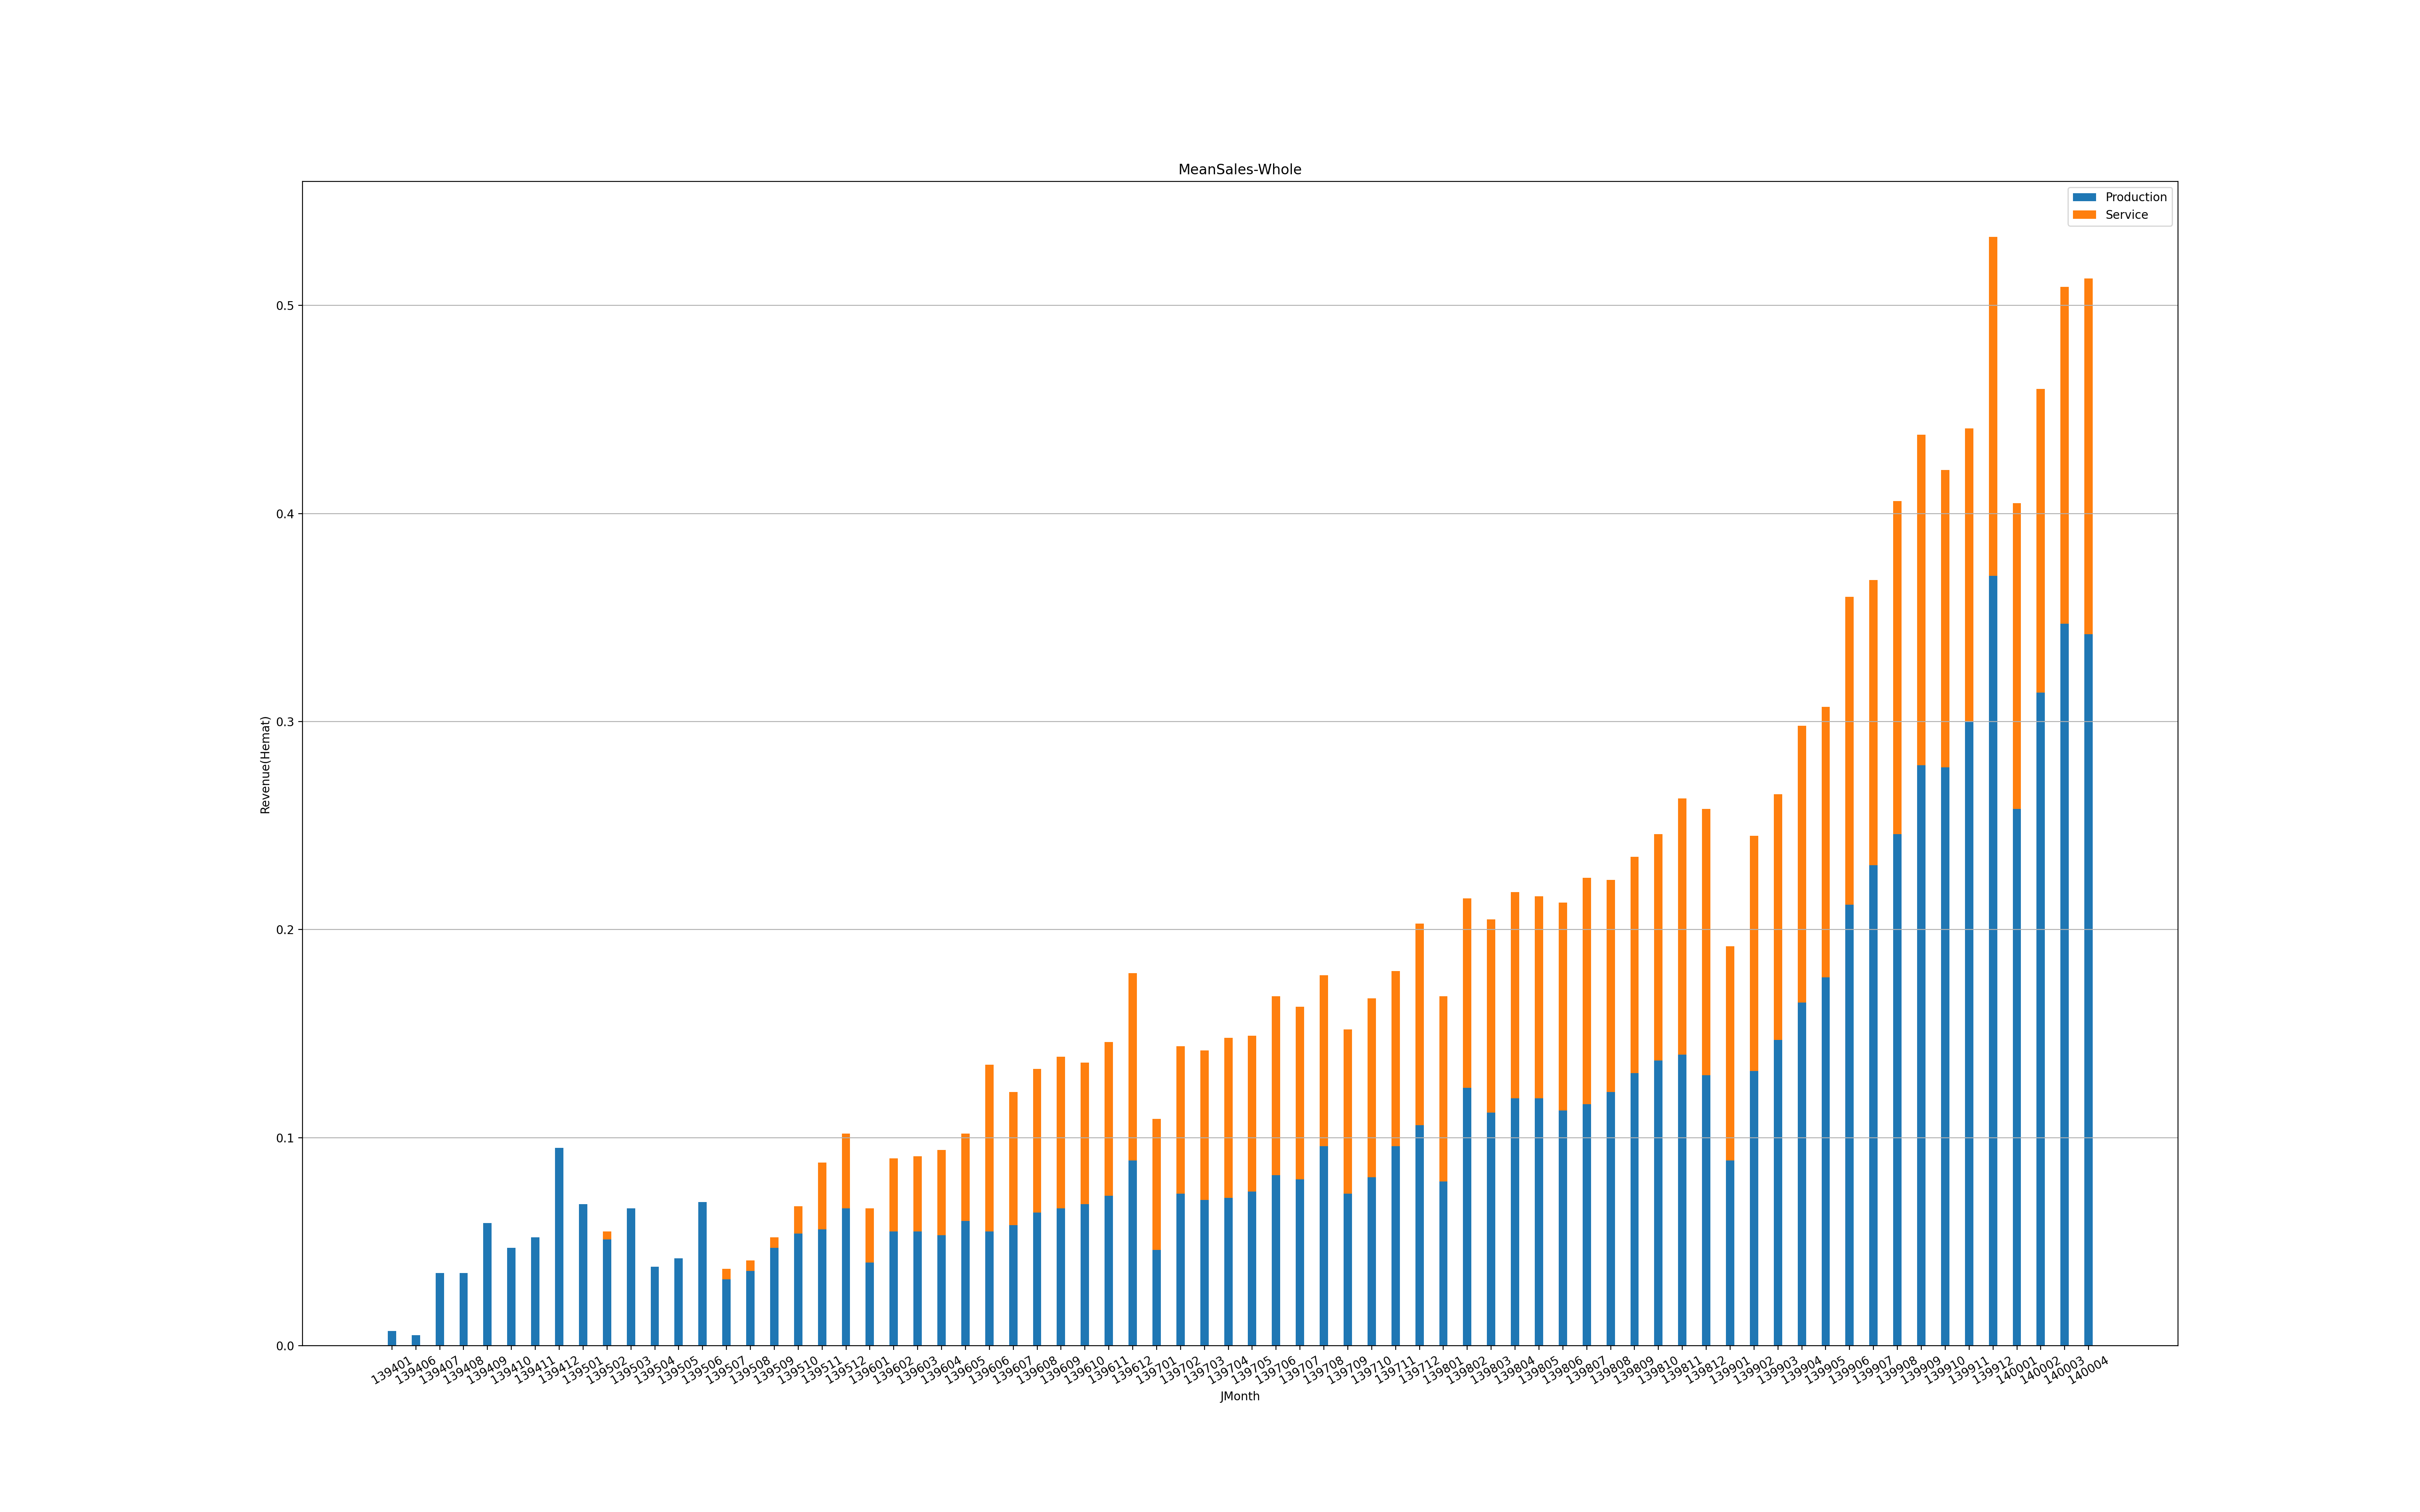
\includegraphics[width=\linewidth]{../data/figs/MeanSales-Whole.png}
    \end{figure}
    \begin{figure}
        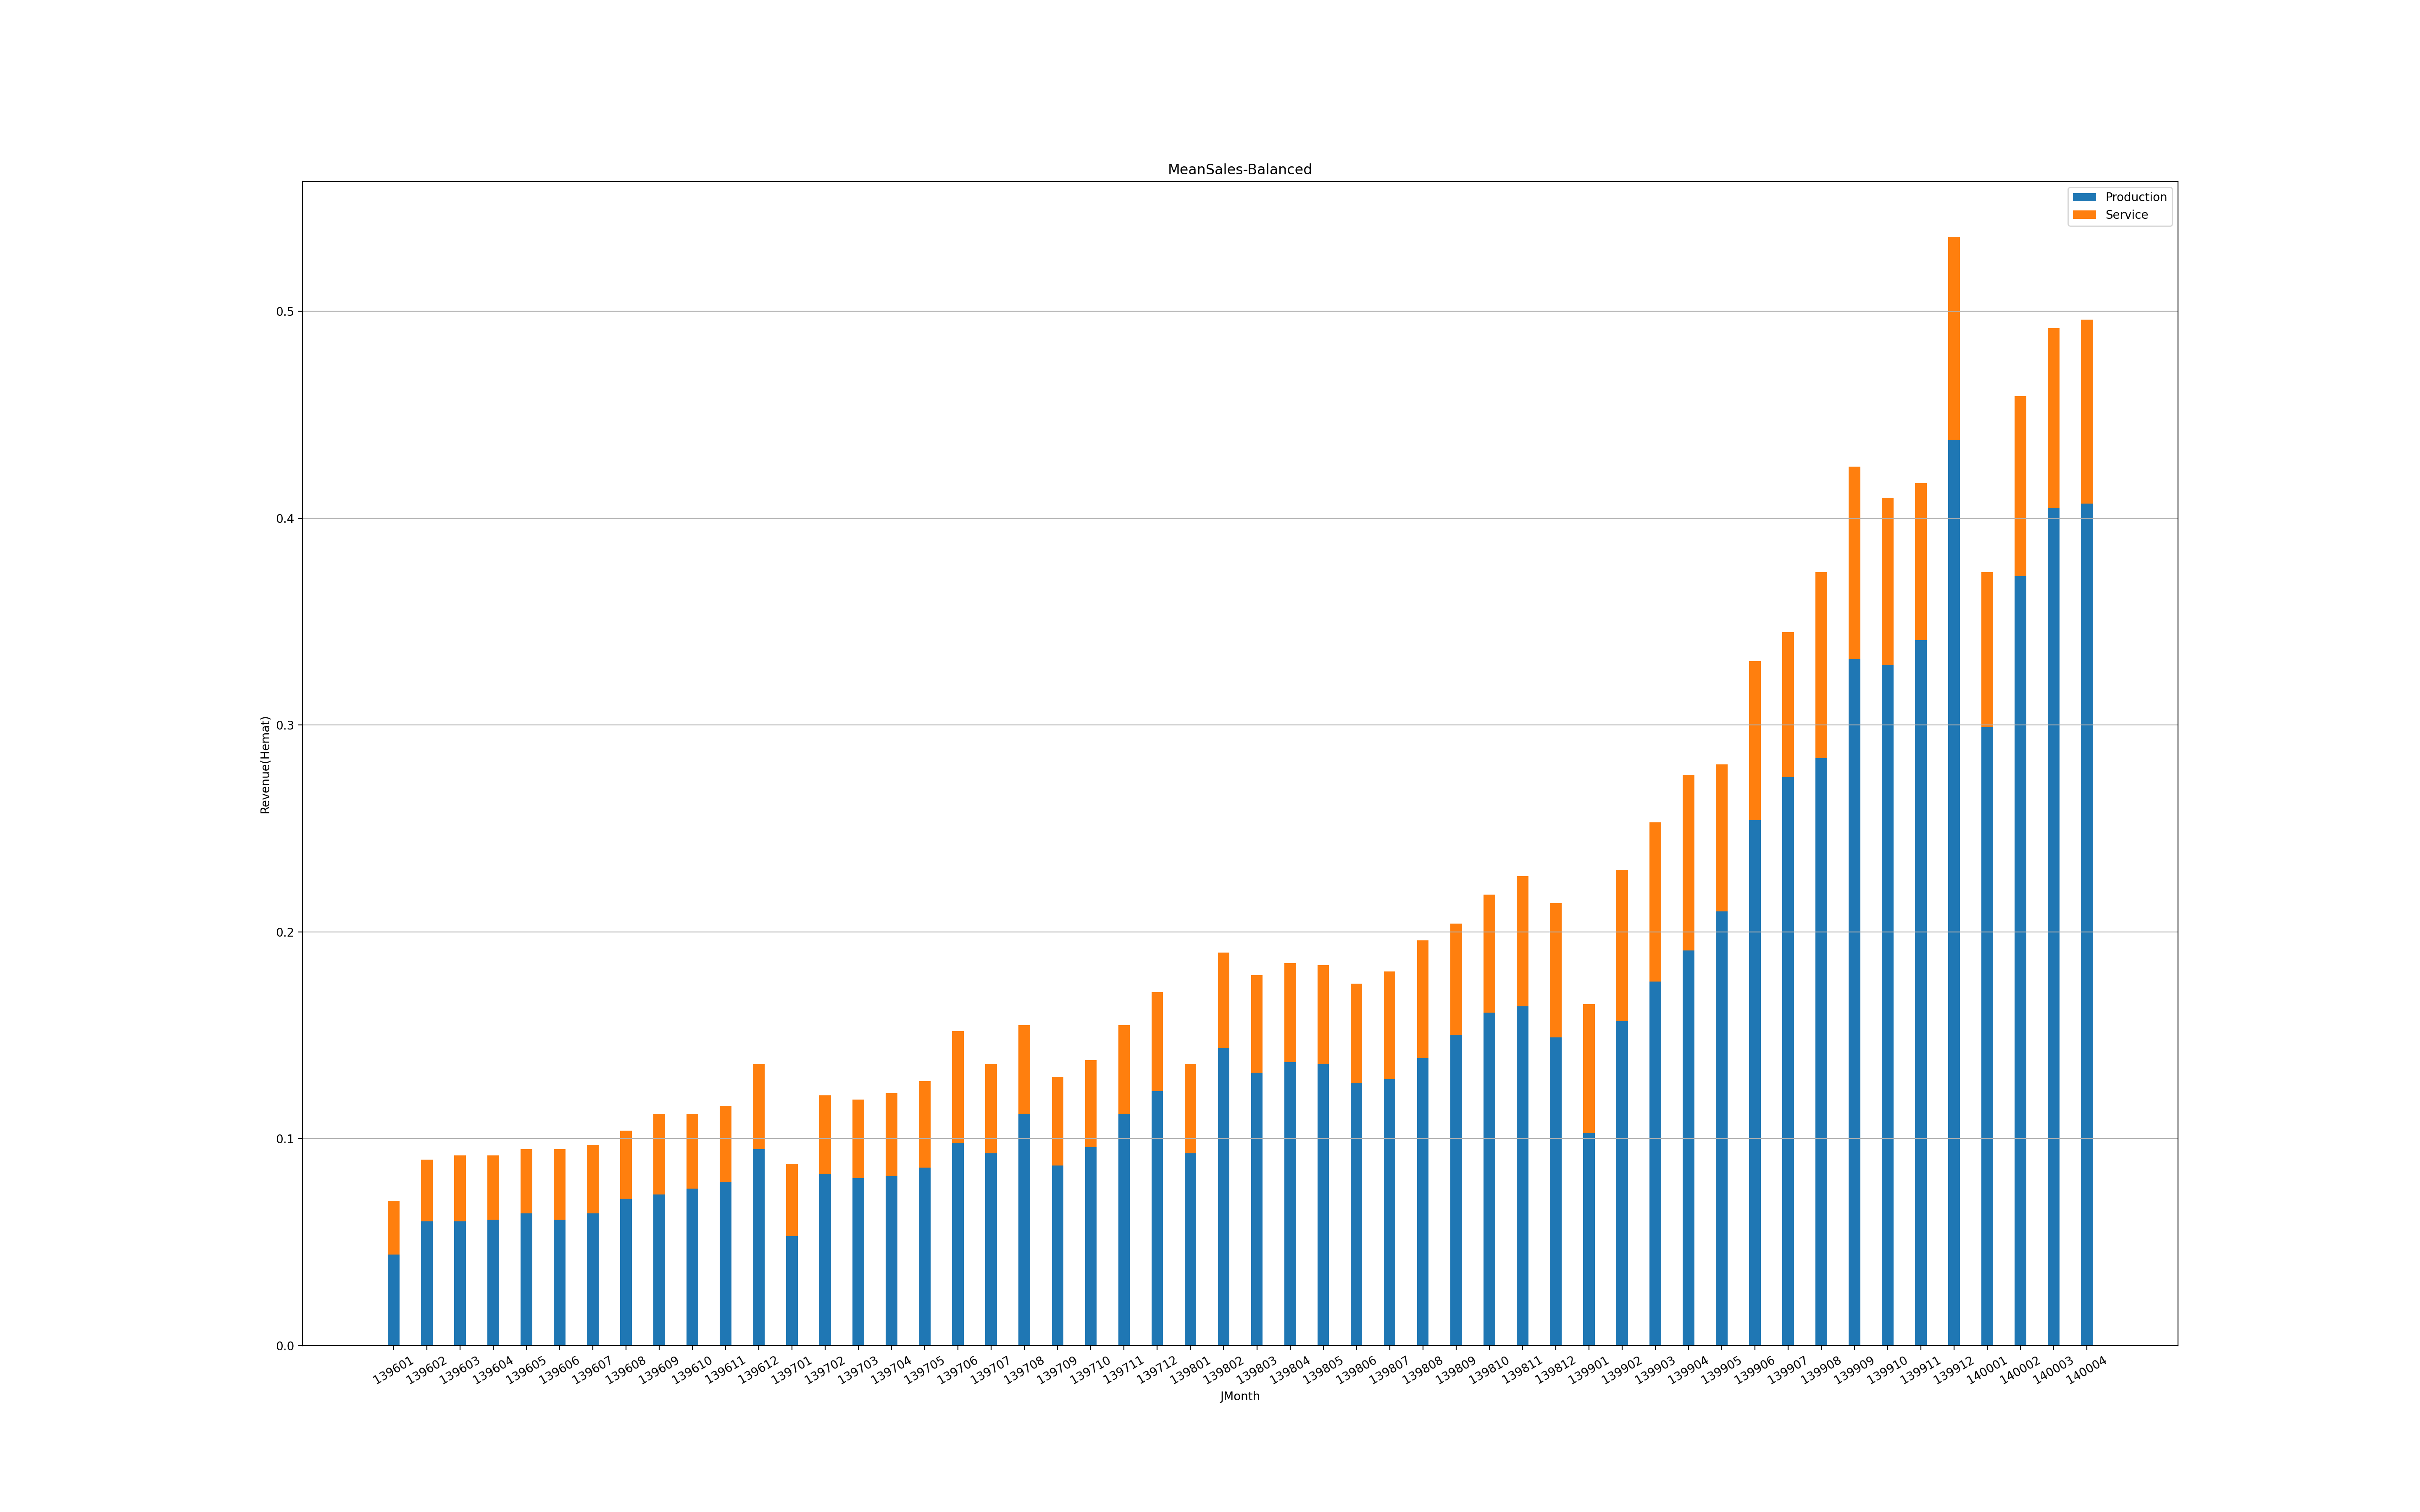
\includegraphics[width=\linewidth]{../data/figs/MeanSales-Balanced.png}
    \end{figure}
    \begin{figure}
        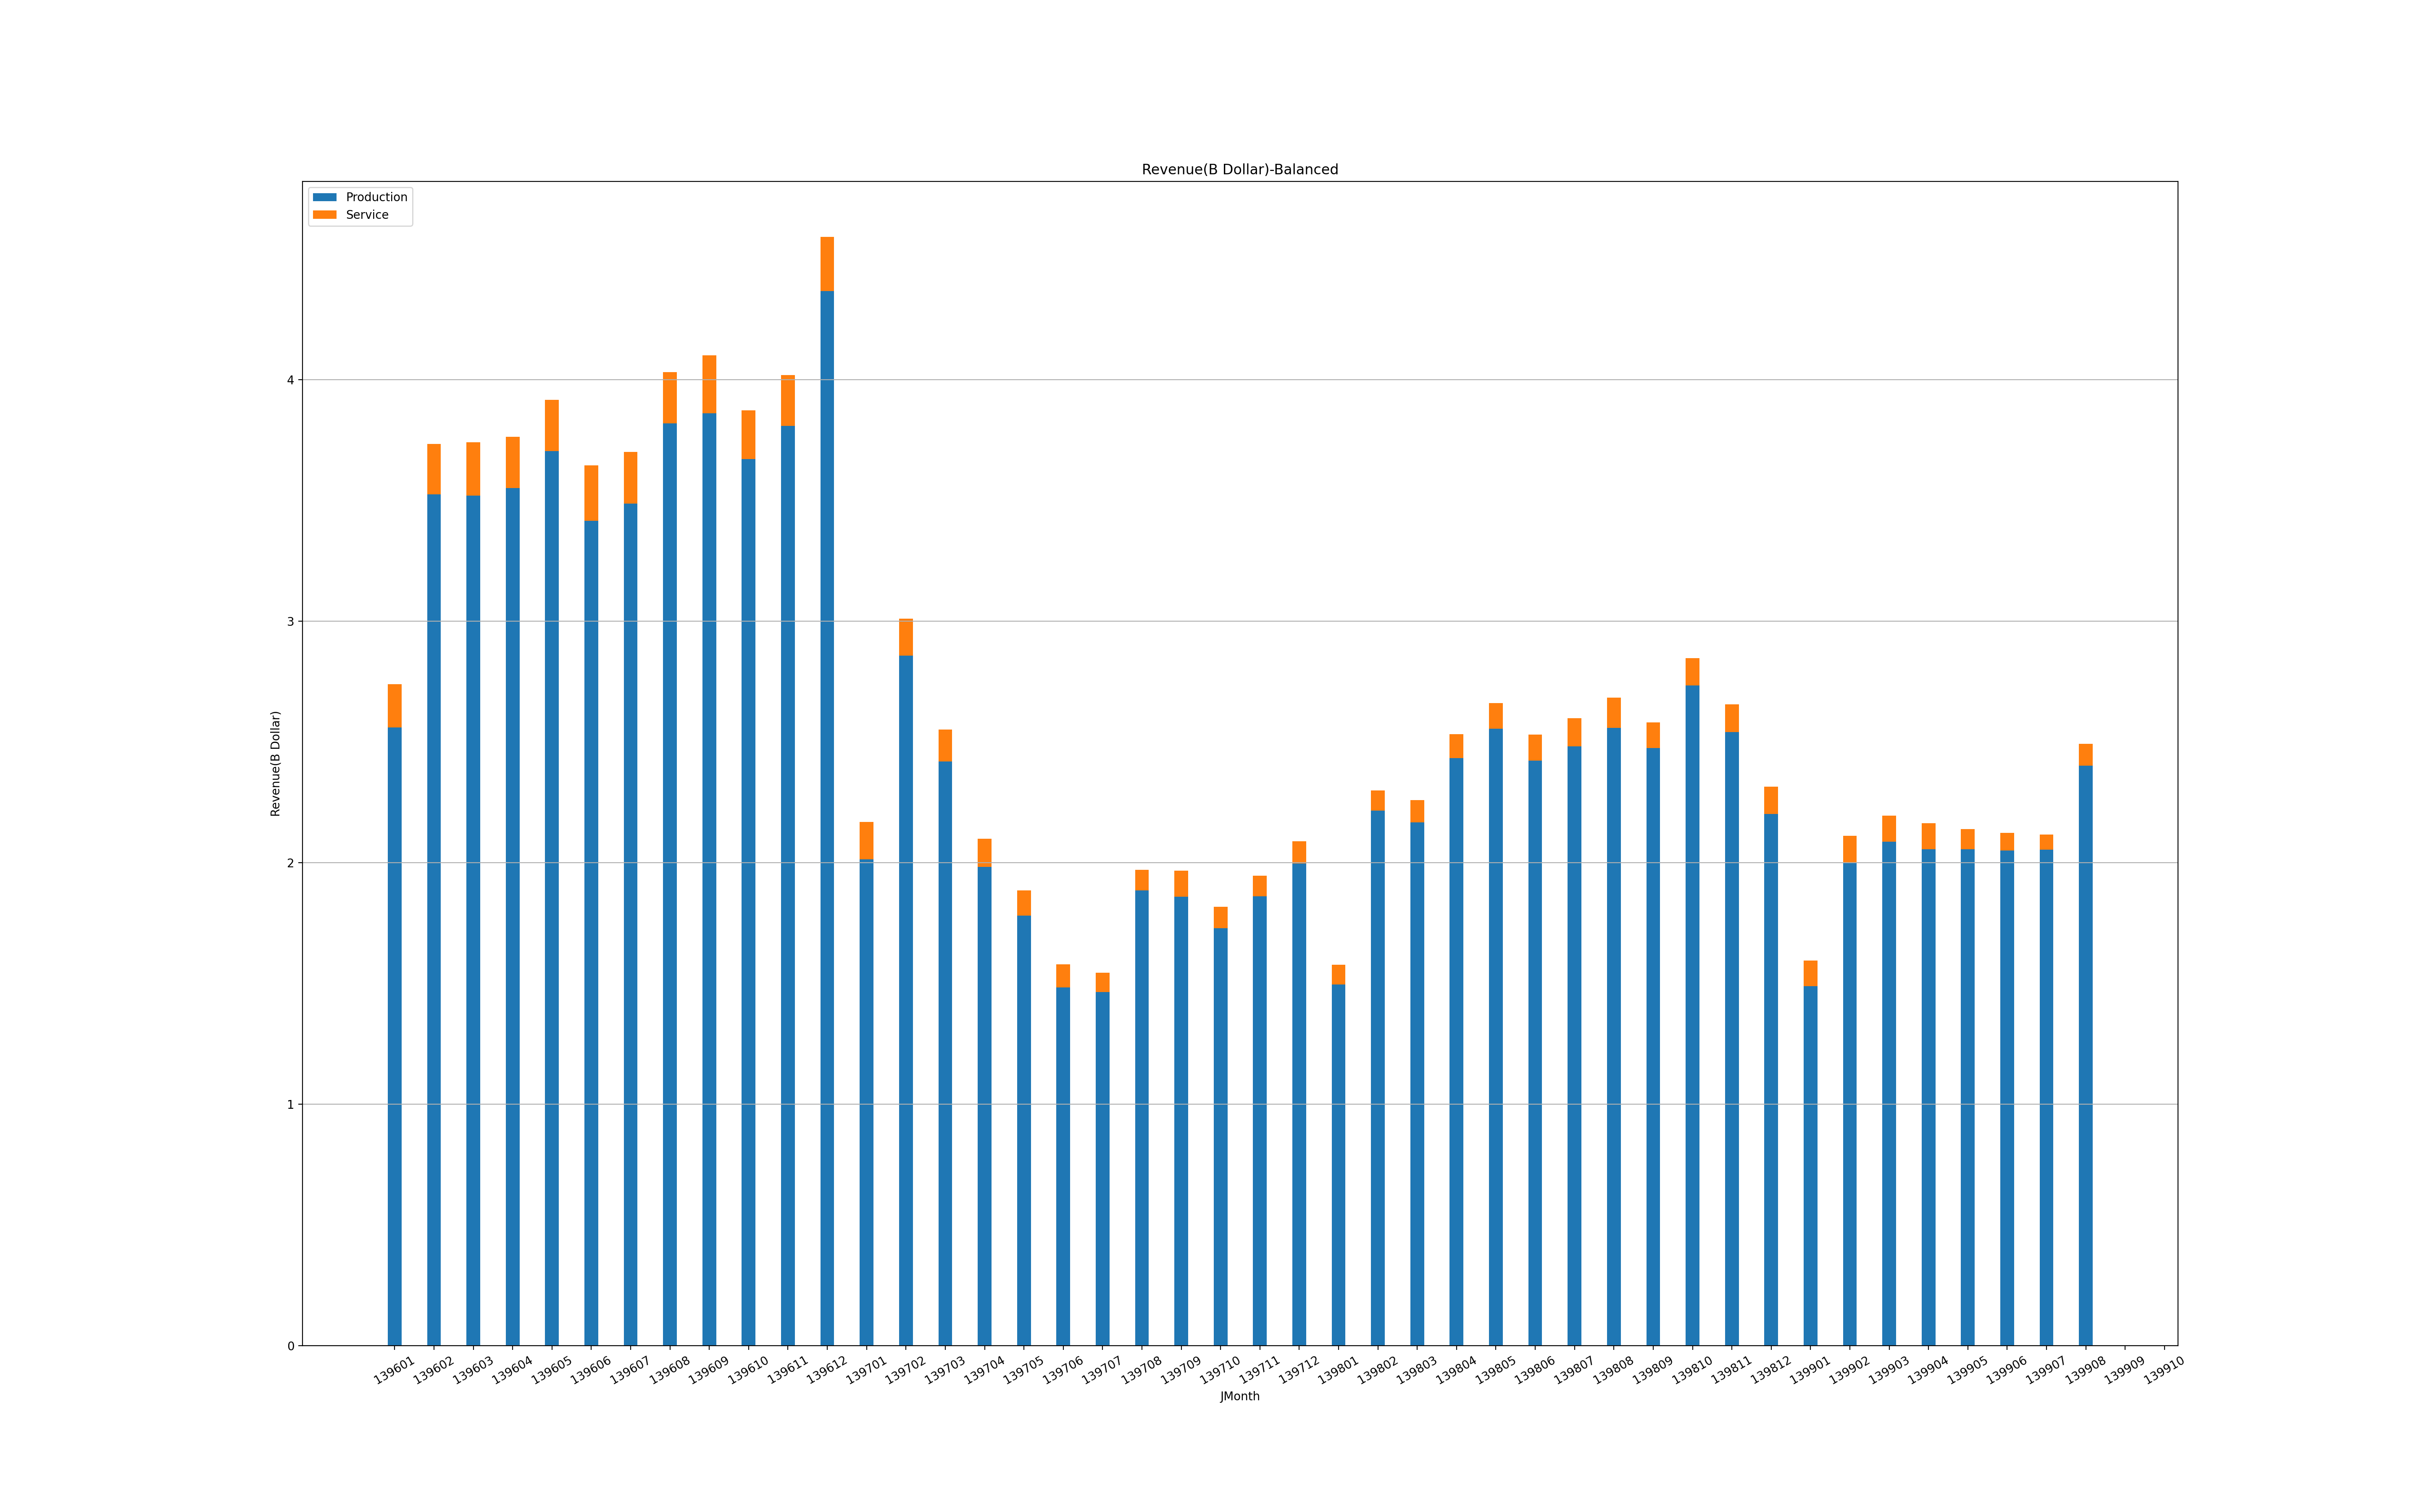
\includegraphics[width=\linewidth]{../data/figs/Revenue(B Dollar)-Balanced.png}
    \end{figure}
    \begin{figure}
        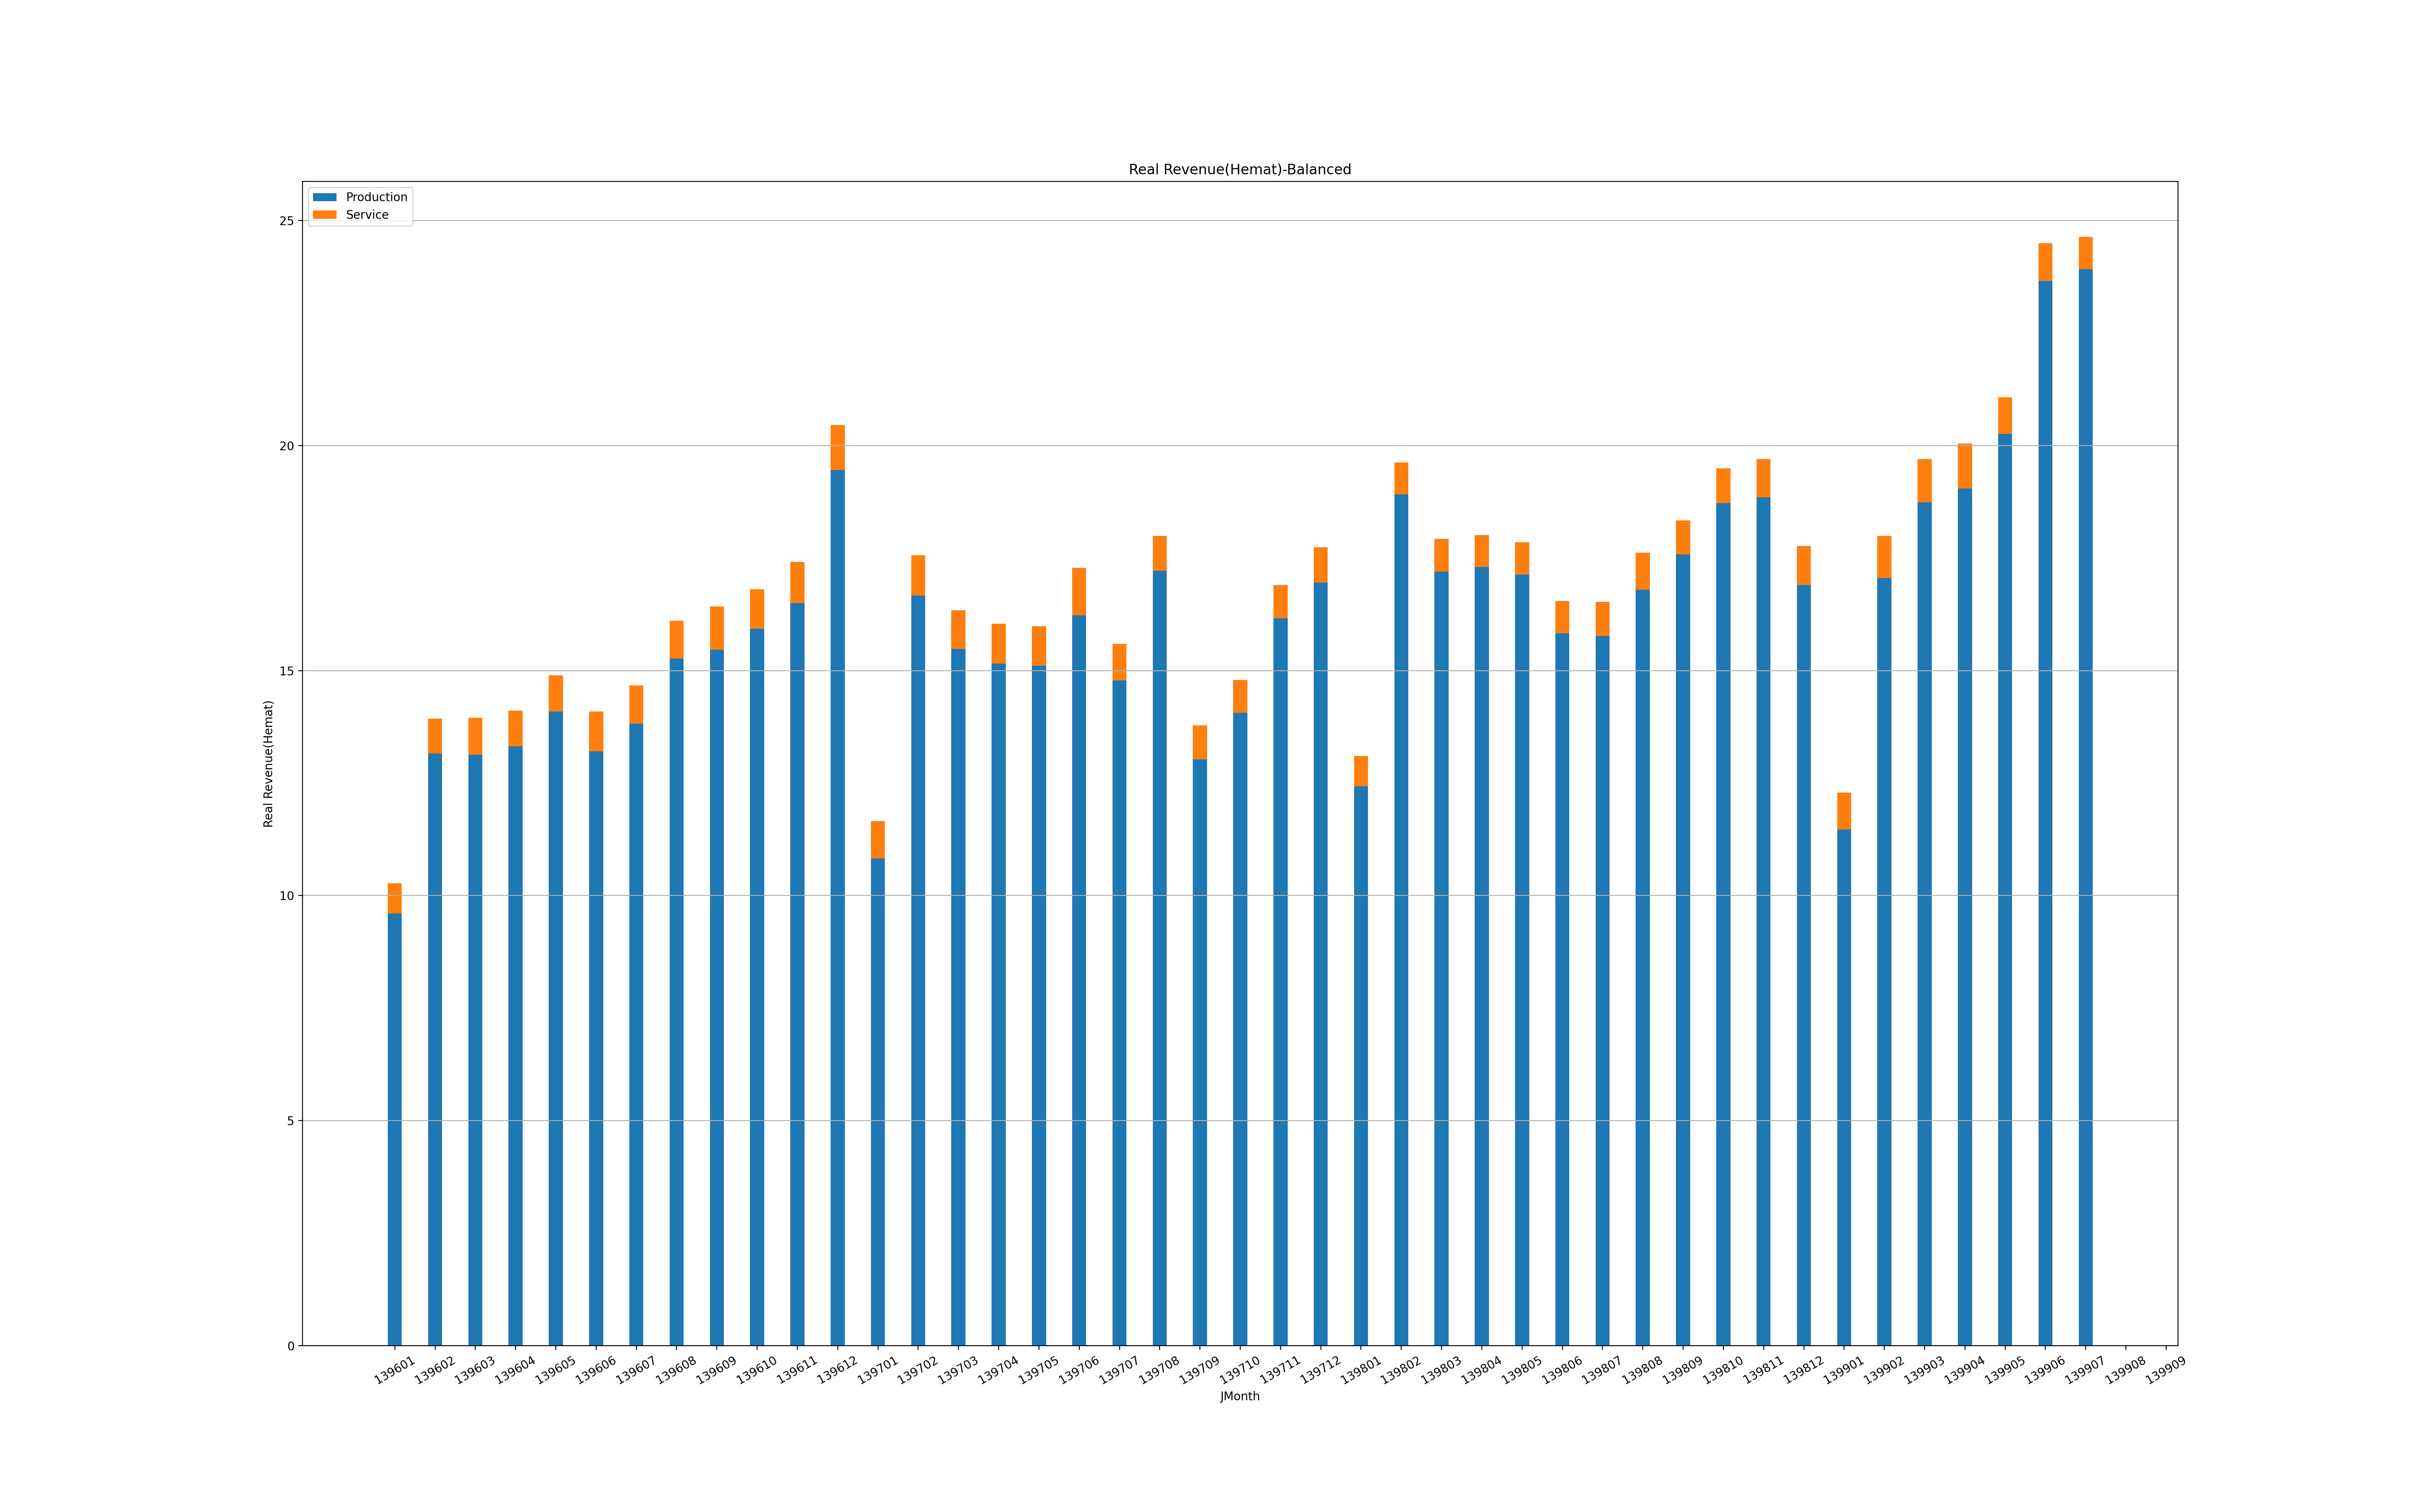
\includegraphics[width=\linewidth]{../data/figs/Real Revenue(Hemat)-Balanced.png}
    \end{figure}
    \begin{figure}
        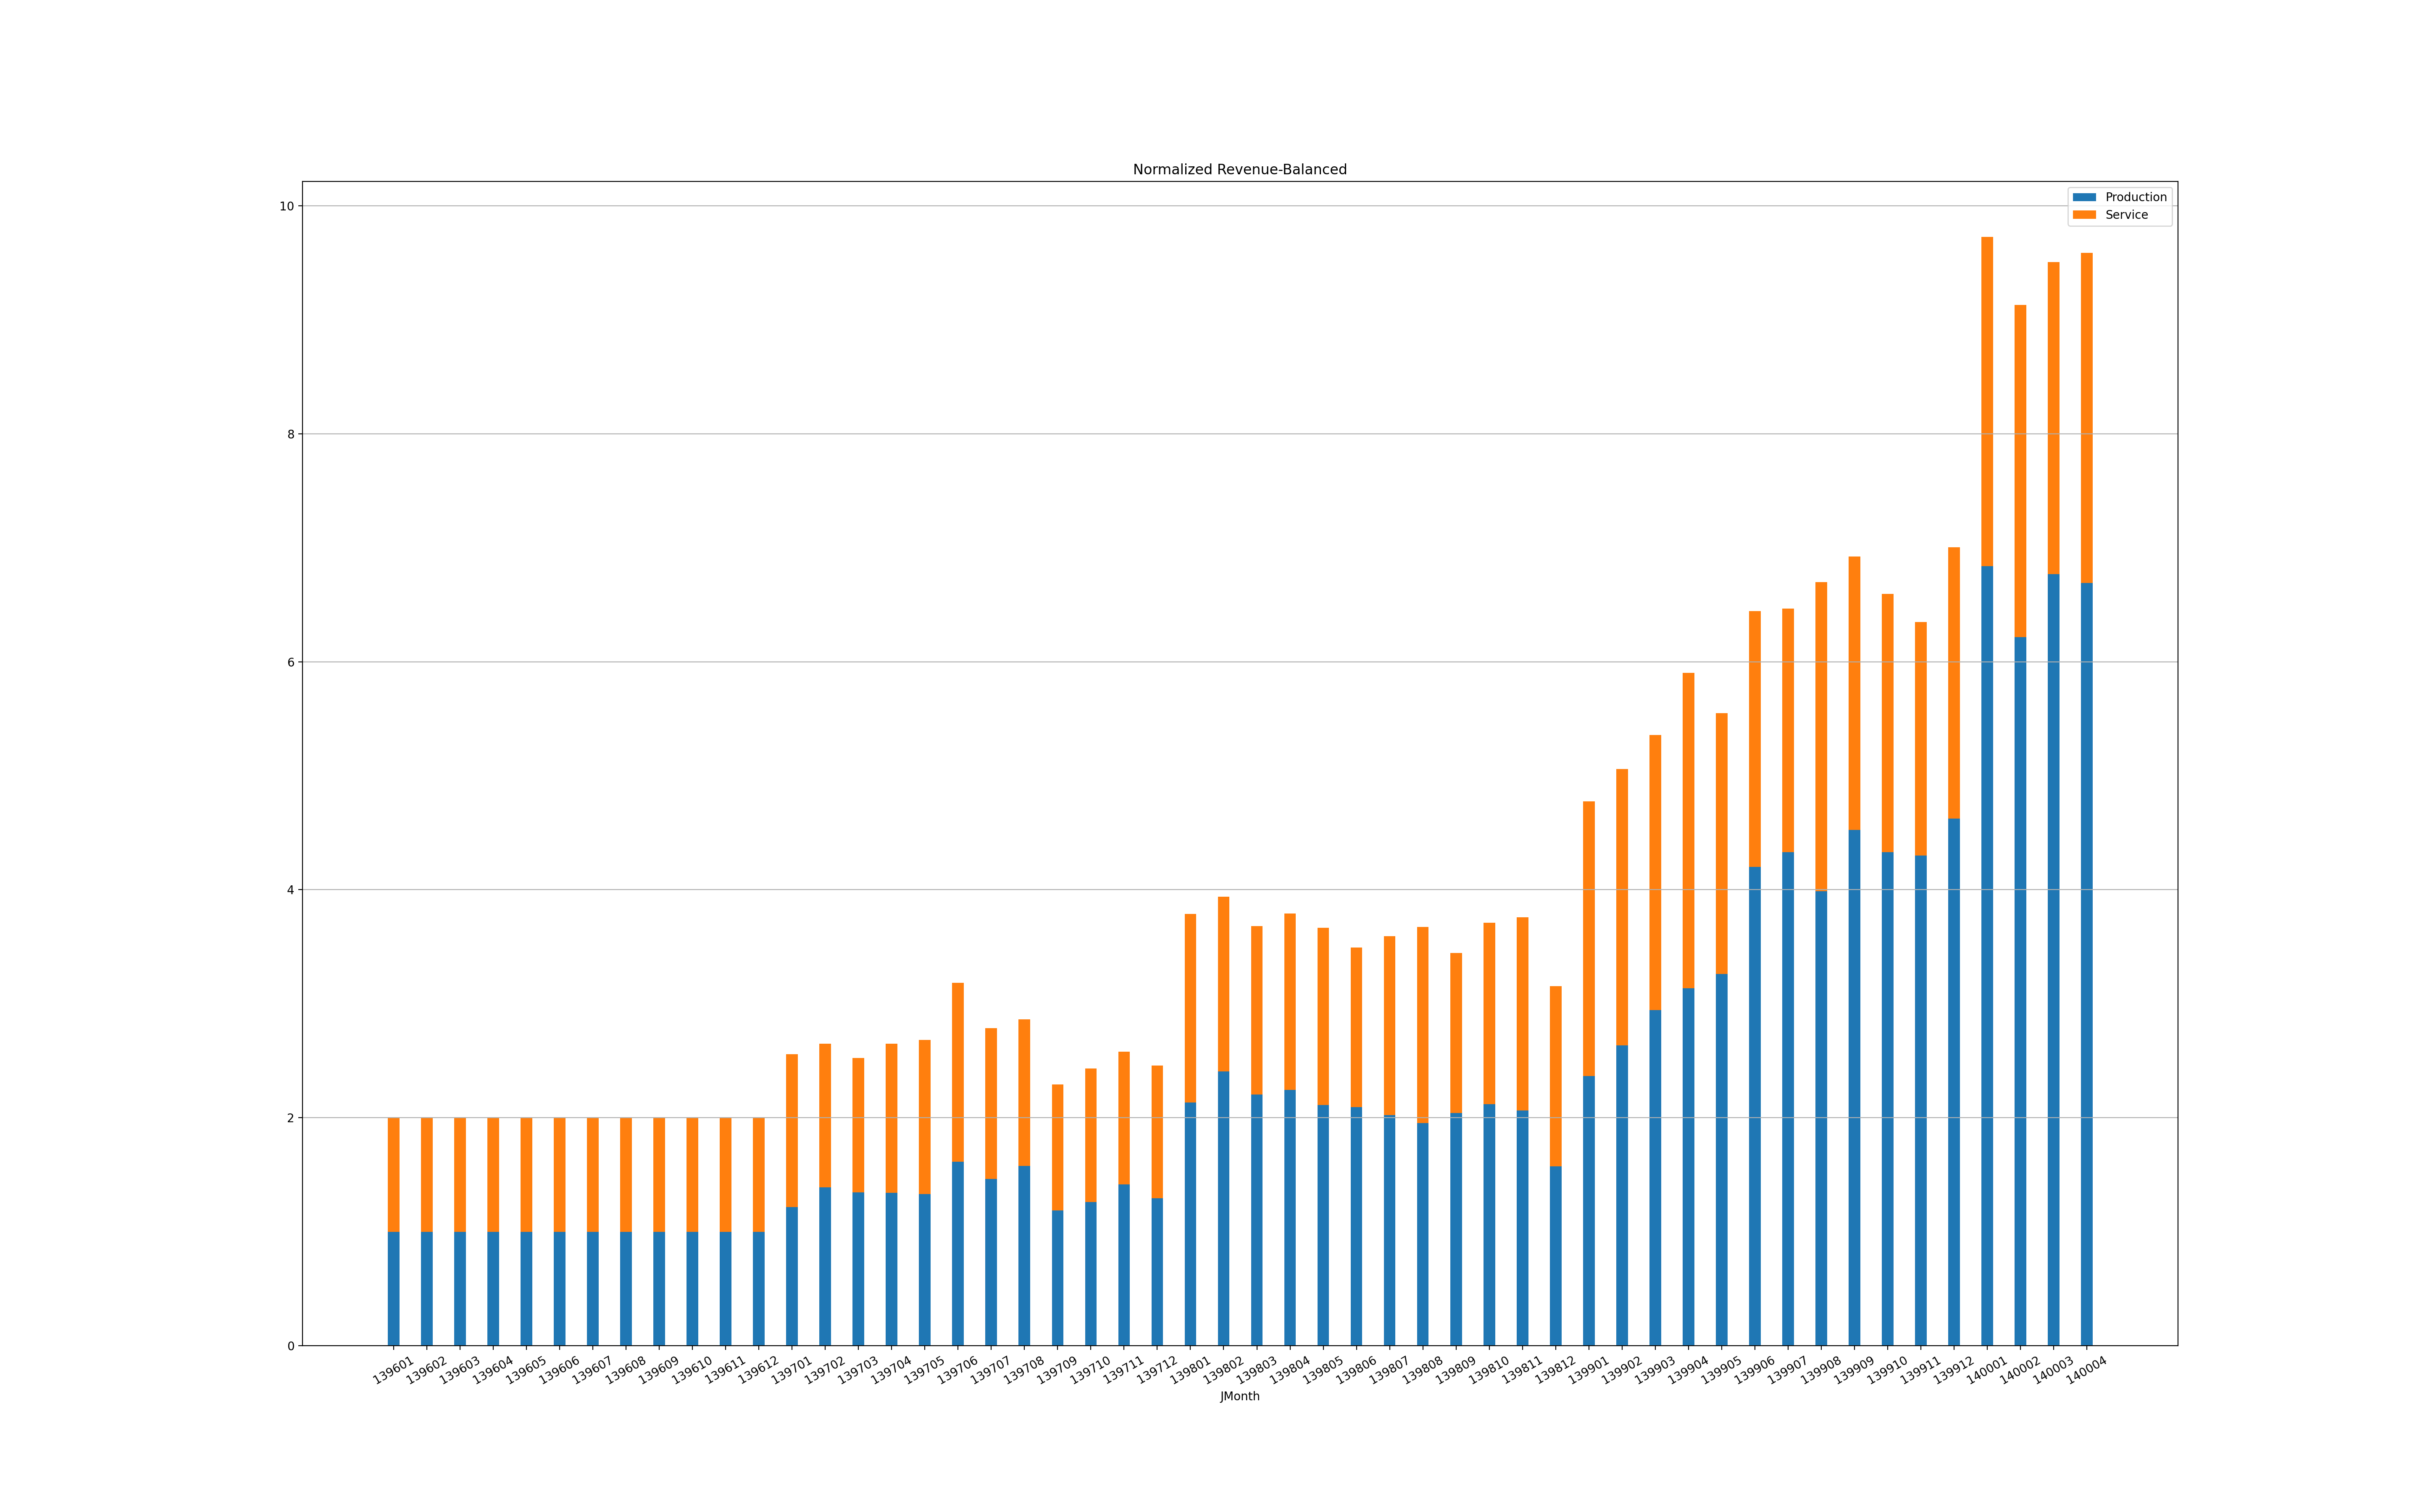
\includegraphics[width=\linewidth]{../data/figs/Normalized Revenue-Balanced.png}
    \end{figure}
    \begin{figure}
        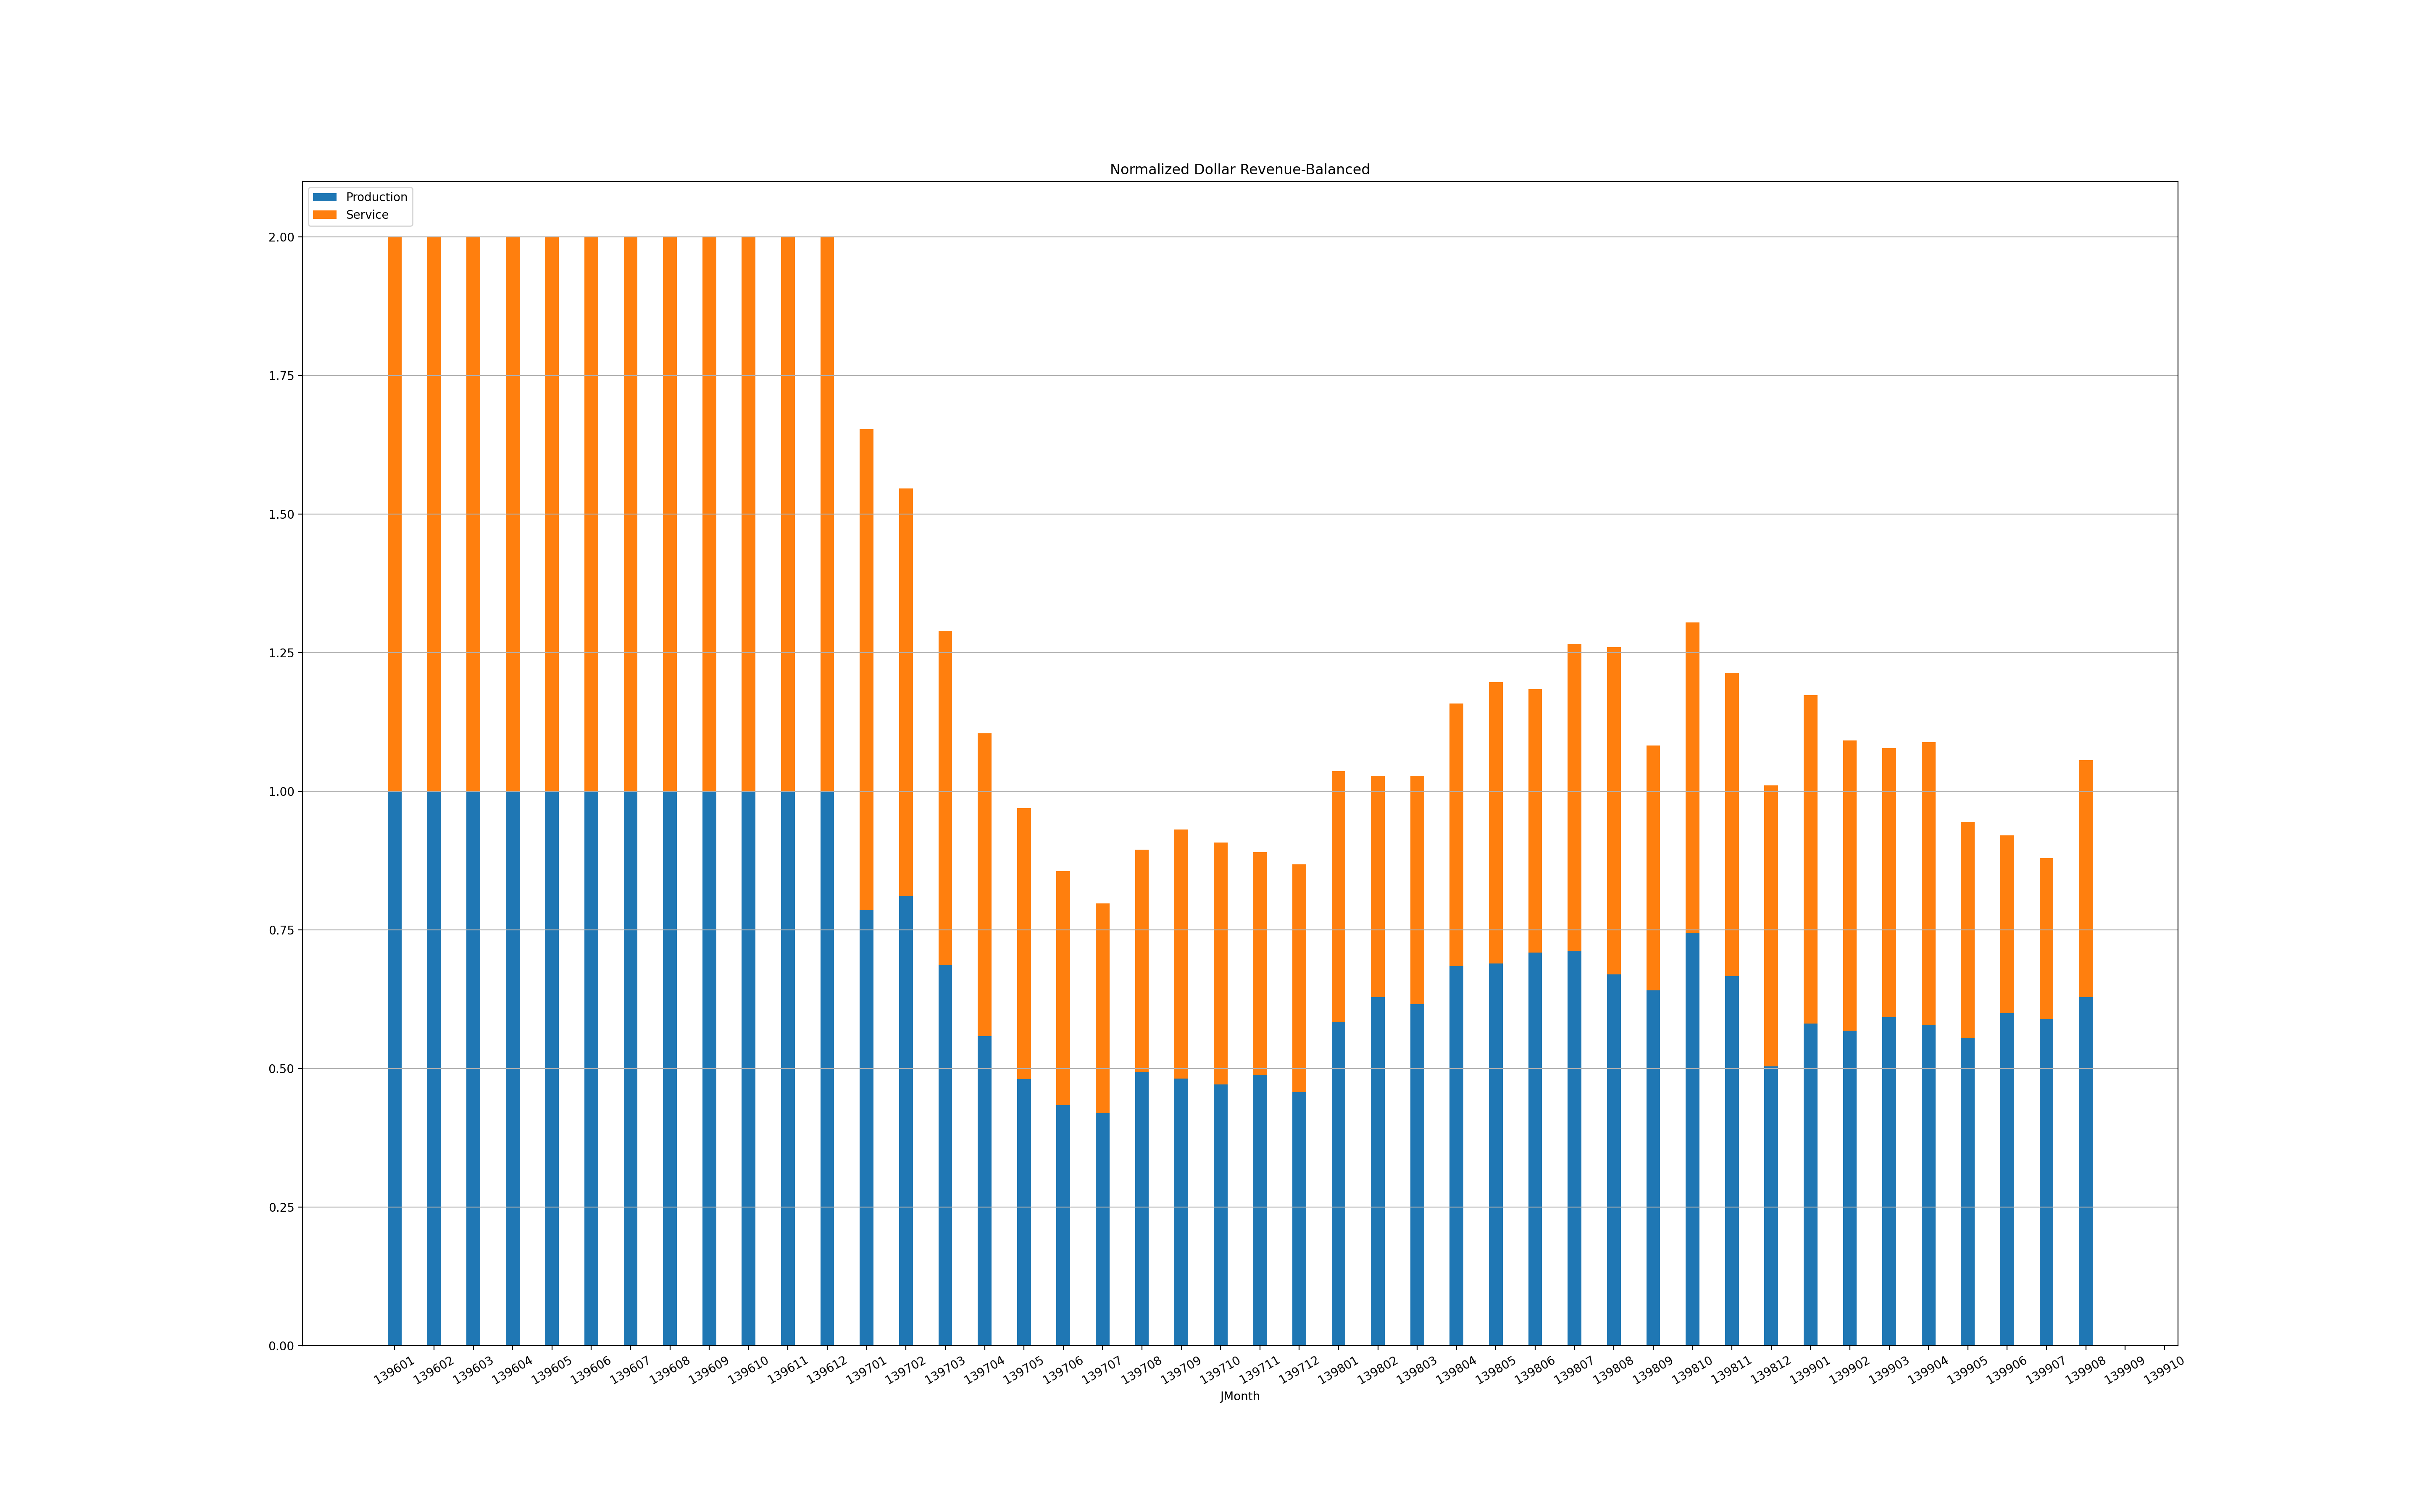
\includegraphics[width=\linewidth]{../data/figs/Normalized Dollar Revenue-Balanced.png}
    \end{figure}
    \begin{figure}
        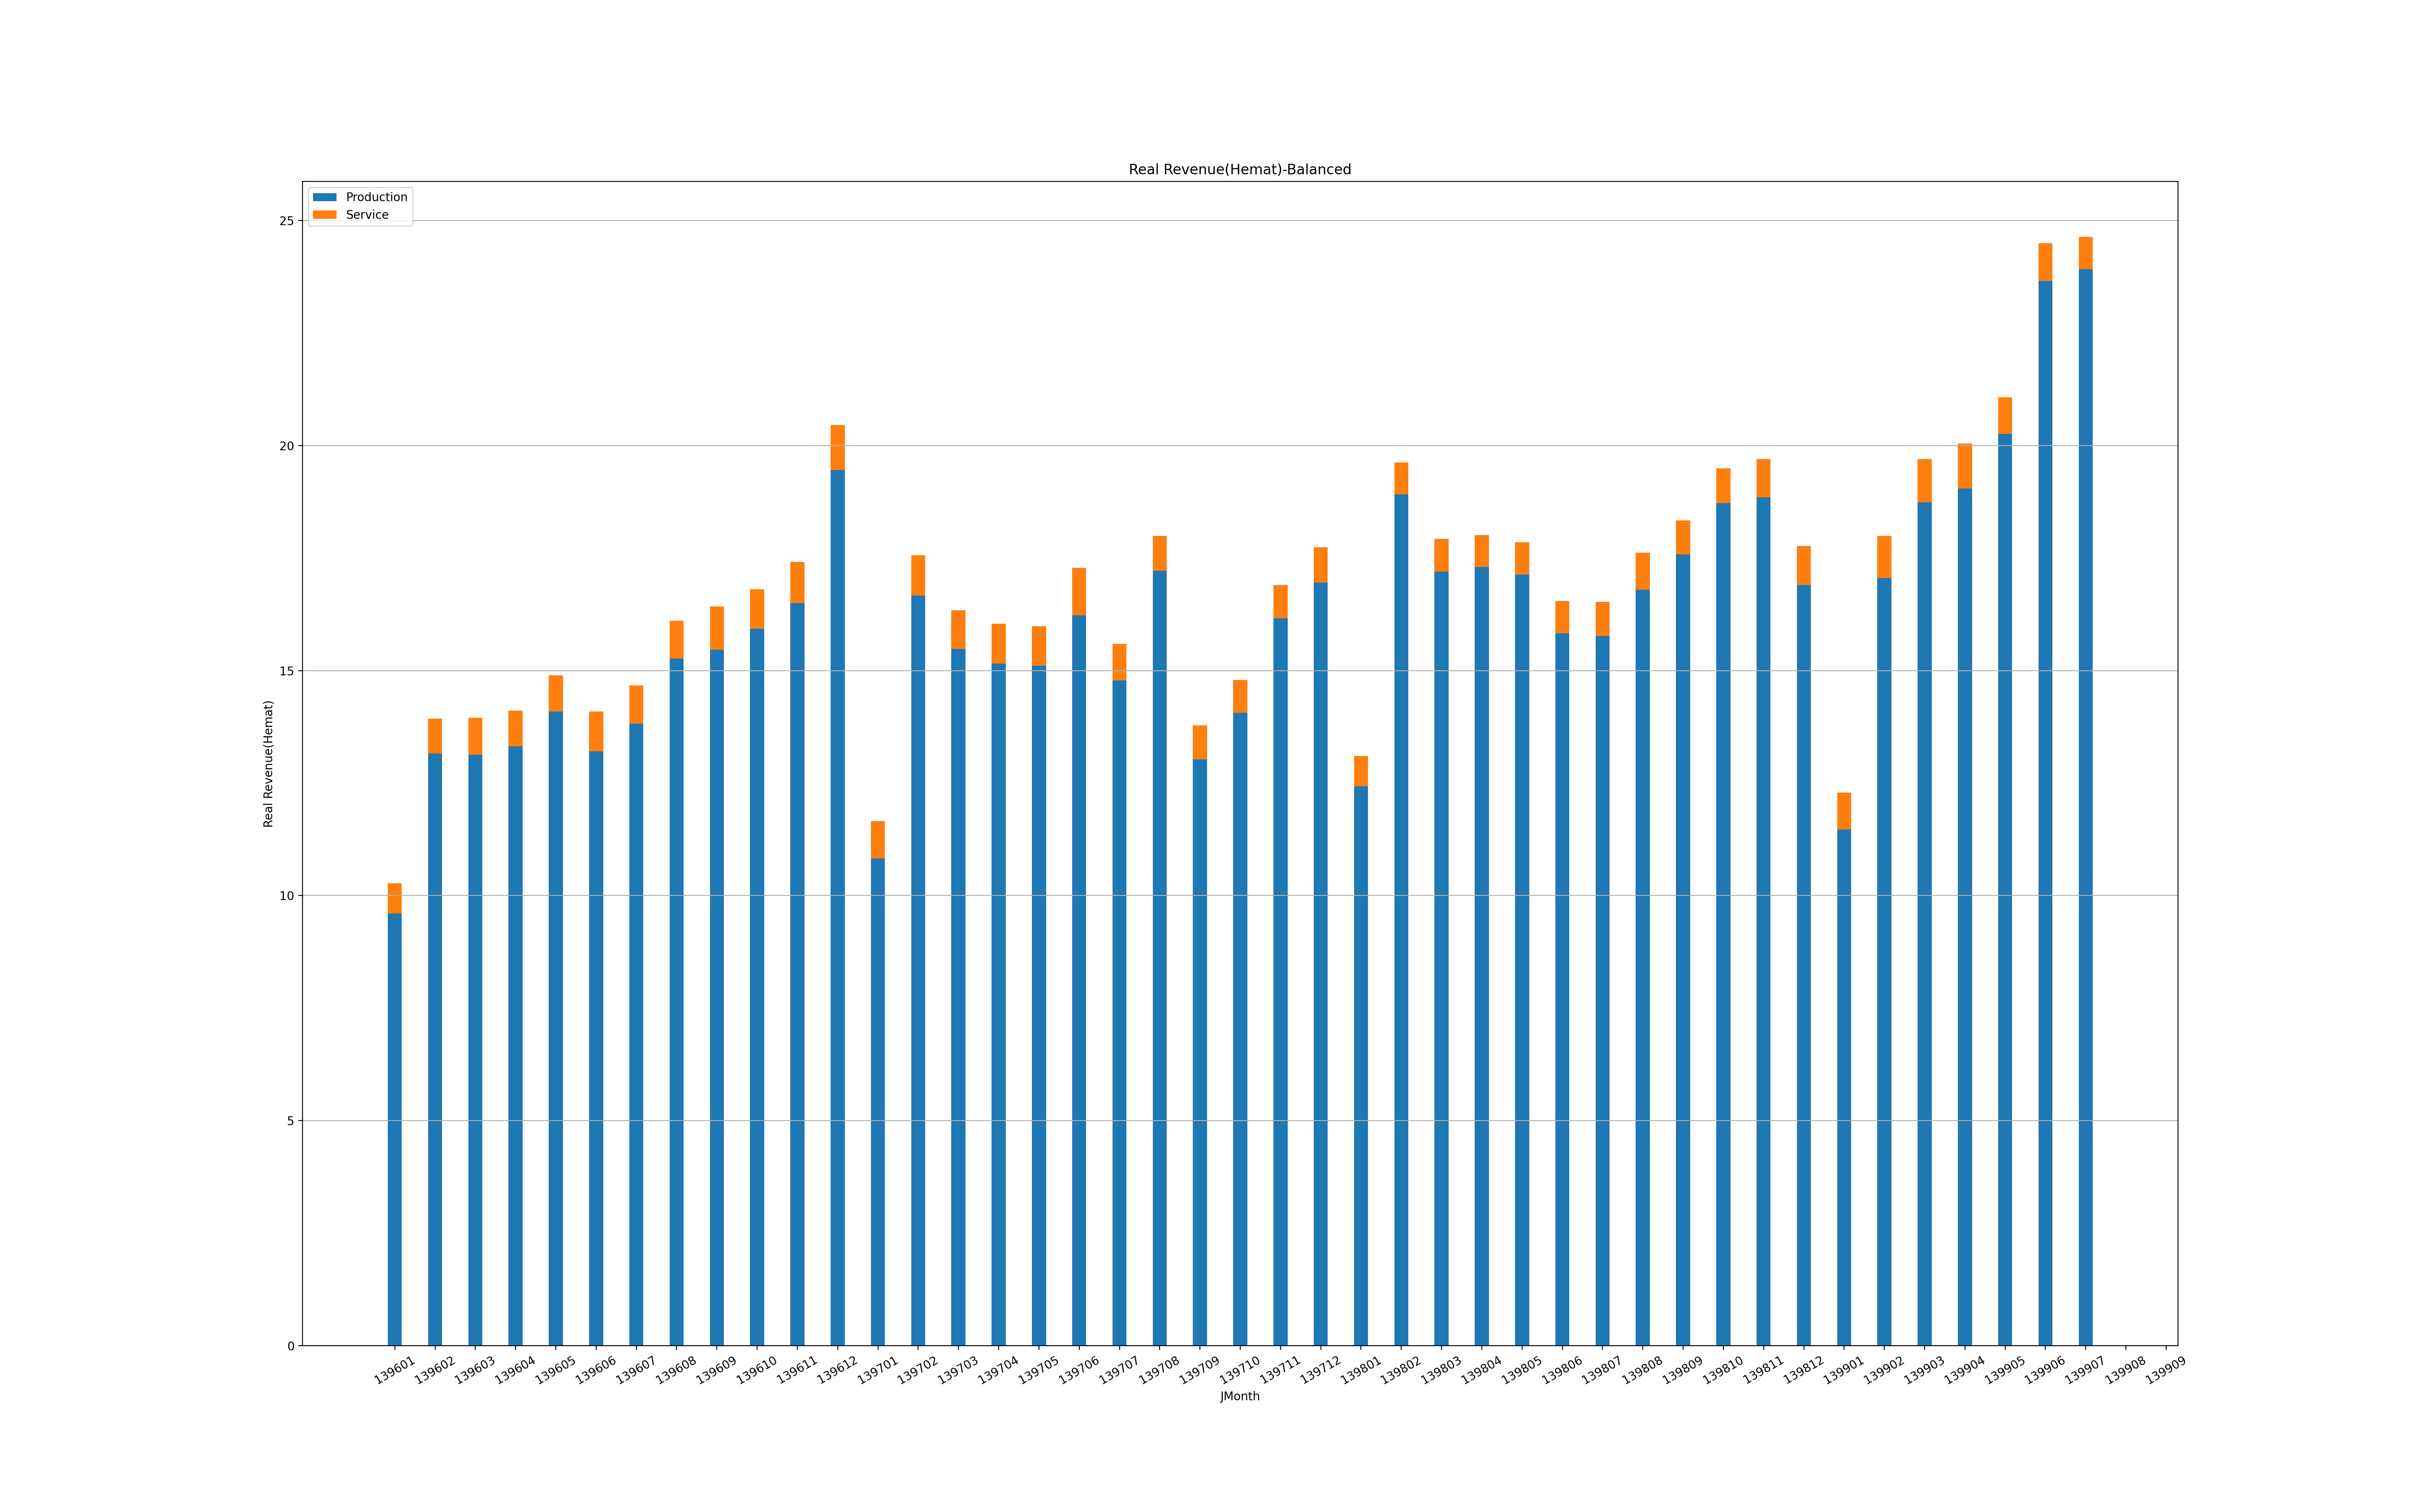
\includegraphics[width=\linewidth]{../data/figs/Real Revenue(Hemat)-Balanced.png}
    \end{figure}


%%%%%%%%%%%%%%%%%%%%%%%%%%%%%%% Document End %%%%%%%%%%%%%%%%%%%%%%%%%%%%%%%%%%
\end{document}
%%%%%%%%%%%%%%%%%%%%%%%%%%%%%%%%%%%%%%%%%%%%%%%%%%%%%%%%%%%%%%%%%%%%%%%%%%%%%%%
